\documentclass[../main.tex]{subfiles}
\begin{document}

\chapter{Grundlagen}
\label{chapter:grundlagen}

\section{Geschichte}
\label{section:geschichte}

1960: Claude Berge

1961: Claude Berge formuliert die Schwache und die Starke Perfekter Graph Vermutung (WPGC und SPGC)

1972: László Lovász beweist die WPGC

1980: 1st Edition vom Buch

Mai 2002: Maria Chudnovsky, Neil Robertson, Paul Seymore und Robin Thomas beweisen die SPGC.

Juni 2002: Claude Berge stirbt.

Nov 2002: Die oben et al. finden einen polynomiellen Algorithmus, um perfekte Graphen zu erkennen.

2004: 2nd Edition vom Buch\cite{das_Buch}

2023: Jun Kawahara et al. releasen ihr Paper über die effiziente Enumeration.

\section{Grundlegende Definitionen}
\label{section:definitionen}

\begin{definition}
    Graph
\end{definition}

Def: die typischen Annahmen für den Kontext (simple, undirected, endlich)

Def Chromatic Number

Rekursives Schema zum berechnen der chromatischen Zahl via Chromatic Polynom

ergo $O(2^{|V|})$

NP-Hardness via Karp's 21 NP-complete problems

Fun Fact: Sudoku ist ein Graph Coloring Problem

Def Clique

Die Chromatische Zahl und die Cliquen-Zahl kann beliebig weit auseinander liegen. Mit der Konstruktion von Jan Myceilski \cite{Mycielski1955} kann man aus einem Graph einen weiteren bauen, sodass die Cliquen-Zahl gleich bleibt, aber die Chromatische Zahl um 1 steigt.

\begin{satz}
    Für alle $n \in \N, n \geq 2$ existiert ein Graph $M_n$ mit $\chi(M_n) = n$ und $\omega(M_n) = 2$.
\end{satz}
\begin{figure}[ht]
    \label{fig:joke}
    \centering
    \includegraphics[width=0.5\textwidth,trim={0 7cm 0 26.5cm},clip]{figures/joke.jpg}
    \caption{Ein vom Myceilskigraphen $M_4$ inspiriertes Bondagemuster. Der Knoten $w$ ist der große mittige Knoten. \todo{remove this lol}}
\end{figure}
\begin{figure}[ht]
    \label{fig:myceilski}
    \centering
    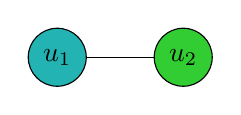
\begin{tikzpicture}[scale=0.8]
        \node[circle, draw, fill=TealBlue] (u1) at (0, 0) {$u_1$};
        \node[circle, draw, fill=LimeGreen] (u2) at (2, 0) {$u_2$};
        \draw (u1) -- (u2);
    \end{tikzpicture}
    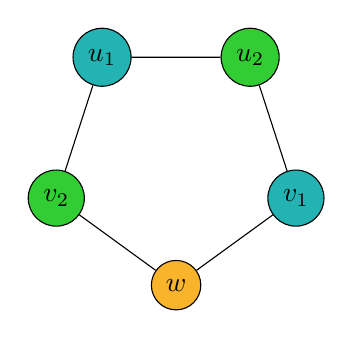
\begin{tikzpicture}[scale=0.8]
        \node[circle, draw, fill=TealBlue ] (c1) at ({126-360/5 * (1 - 1)}:2) {$u_1$};
        \node[circle, draw, fill=LimeGreen] (c2) at ({126-360/5 * (2 - 1)}:2) {$u_2$};
        \node[circle, draw, fill=TealBlue ] (c3) at ({126-360/5 * (3 - 1)}:2) {$v_1$};
        \node[circle, draw, fill=Dandelion] (c4) at ({126-360/5 * (4 - 1)}:2) {$w$};
        \node[circle, draw, fill=LimeGreen] (c5) at ({126-360/5 * (5 - 1)}:2) {$v_2$};
        
        \foreach \i in {1, 2, 3, 4, 5} {
            \pgfmathtruncatemacro{\j}{mod(\i, 5) + 1}
            \draw (c\i) -- (c\j);
        }
    \end{tikzpicture}
    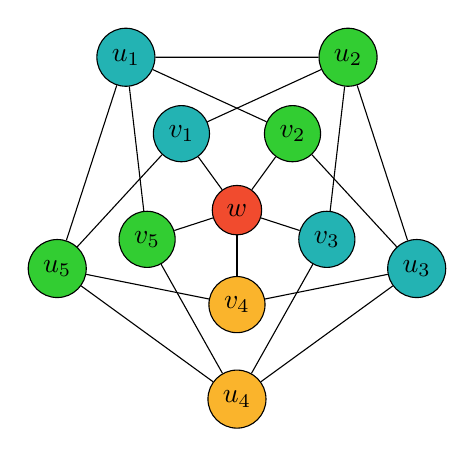
\begin{tikzpicture}[scale=0.8]        
        \node[circle, draw, fill=TealBlue ] (u1) at ({126-360/5 * (1 - 1)}:3) {$u_1$};
        \node[circle, draw, fill=LimeGreen] (u2) at ({126-360/5 * (2 - 1)}:3) {$u_2$};
        \node[circle, draw, fill=TealBlue ] (u3) at ({126-360/5 * (3 - 1)}:3) {$u_3$};
        \node[circle, draw, fill=Dandelion] (u4) at ({126-360/5 * (4 - 1)}:3) {$u_4$};
        \node[circle, draw, fill=LimeGreen] (u5) at ({126-360/5 * (5 - 1)}:3) {$u_5$};
        \foreach \i in {1, 2, 3, 4, 5} {
            \pgfmathtruncatemacro{\j}{mod(\i, 5) + 1}
            \draw (u\i) -- (u\j);
        }
        \node[circle, draw, fill=TealBlue ] (v1) at ({126-360/5 * (1 - 1)}:1.5) {$v_1$};
        \node[circle, draw, fill=LimeGreen] (v2) at ({126-360/5 * (2 - 1)}:1.5) {$v_2$};
        \node[circle, draw, fill=TealBlue ] (v3) at ({126-360/5 * (3 - 1)}:1.5) {$v_3$};
        \node[circle, draw, fill=Dandelion] (v4) at ({126-360/5 * (4 - 1)}:1.5) {$v_4$};
        \node[circle, draw, fill=LimeGreen] (v5) at ({126-360/5 * (5 - 1)}:1.5) {$v_5$};

        \node[circle,  draw, fill=RedOrange] (w) at (0, 0) {$w$};
        \foreach \i in {1, 2, 3, 4, 5} {
            \pgfmathtruncatemacro{\j}{mod(\i, 5) + 1}
            \pgfmathtruncatemacro{\k}{mod(\i+3, 5) + 1}
            \draw (u\j) -- (v\i);
            \draw (u\k) -- (v\i);
            \draw (v\i) -- (w);
        }
    \end{tikzpicture}
    \caption{Die ersten drei Myceilski-Graphen: $M_2 = K_2, M_3 = C_5, M_4$}
\end{figure}
\begin{proof}
    per Induktion: für $n = 2$ erfüllt der Graph $M_2 := K_2$ mit 2 Knoten und einer Kante das gewünschte.
    für $n > 2$ sei also $M_{n-1}$ (mit $m$ Knoten) gegeben und seien $u_1, \hdots, u_m$ die Knoten von $M_{n-1}$. Wir definieren zuerst $M_n$ und zeigen dann, dass $M_n$ die gewünschten Eigenschaften hat.

    $M_n$ soll $M_{n-1}$ als Teilgraphen enthalten, sowie $m+1$ extra Knoten: einen Knoten $v_i$ pro Knoten $u_i$ sowie einen Extraknoten $w$. Für jede Kante $u_iu_j$ in $M_{n-1}$ gibt es drei Kanten in $M_n$: Die originale Kante $u_iu_j$ selbst sowie $u_iv_j$ und $v_iu_j$. Des weiteren sind gibt es zu jedem neuen Knoten $v_i$ die Kante $v_iw$. Das sind alle\footnote{Au$\star$ intensifies} Kanten.
    
    Z.z. $\omega(M_n) = 2$: Wir wollen also zeigen, dass es keine Cliquen der Größe 3, i.e. Dreiecke gibt. Wir betrachten Tripel von Knoten und unterscheiden nach der Kategorie der Knoten:
    \begin{itemize}
        \item $(w, u_i, v_j)$ oder $(w, u_i, u_j)$: $w$ ist nicht mit den Originalknoten $u_i$ verbunden, also ist dies kein Dreieck.
        \item $(w, v_i, v_j)$ oder $(v_i, v_j, u_k)$ oder $(v_i, v_j, v_k)$: Die Knoten $v_i$ sind nicht untereinander verbunden, also ist auch dies kein Dreieck.
        \item $(u_i, u_j, u_k)$: Aufgrund der Induktionsvorraussetzung ist $M_{n-1}$ dreieckfrei, also ist auch dies kein Dreieck.
        \item $(u_i, u_j, v_k)$: Ist $k=i$ (bzw. $k=j$), dann ist $u_i$ (bzw. $u_j$) und $v_k$ nicht verbunden. Andernfalls ist $(u_i, u_j, v_k)$ genau dann ein Dreieck, wenn $(u_i, u_j, u_k)$ eines ist. Dies ist laut Induktionsvorraussetzung nicht der Fall.
    \end{itemize}
    Damit ist $\omega(M_n) = 2$ gezeigt.

    Z.z. $\chi(M_n) \geq n$: Angenommen es gibt ein Coloring $c$ mit $n-1$ Farben, o.B.d.A. mit $c(w) = n-1$. Da $w$ mit allen Knoten $v_i$ verbunden ist, gilt $c(v_i) \neq n-1$. Wir definieren eine neue Färbung $c'$ von $M_{n-1}$ mit $n-2$ Farben.
    \begin{align*}
        c' : M_{n-1} &\to \N_{\leq n-2} \\
        u_i &\mapsto \begin{cases}
            c(v_i) &c(u_i) = n-1 \\
            c(u_i) &sonst
        \end{cases}
    \end{align*}

    Nach Konstruktion von $M_n$ sind die Nachbaren von $u_i$ alle mit $v_i$ benachbart, also ist $c'$ eine zulässige Färbung mit $n-2$ Farben, ein Widerspruch zur Induktionsannahme.

    Z.z. $\chi(M_n) \leq n$: Mit einer zulässigen Färbung $c'$ von $M_{n-1}$ mit $n-1$ Farben, lässt sich einfach eine zulässige Färbung $c$ von $M_n$ mit $n$ Farben definieren:
    \begin{align*}
        c : M_n &\to \N_{\leq n} \\
        c(u_i) &:= c'(u_i) \\
        c(v_i) &:= c'(u_i) \\
        c(w) &:= n
    \end{align*}

    Damit gilt also zusammengefasst $\chi(M_n) = n$.
\end{proof}

Die so konstruierten Graphen werden \emph{Myceilski-Graphen} genannt. In Abbildung \ref{fig:myceilski} sind die ersten drei Myceilskigraphen mit der Färbung $c$ aus dem letzten Beweisschritt dargestellt.

\section{Perfekte Graphen}

Def Perfekter Graph

%Reduktionsschema bzw. Induktion nach Knotenanzahl:
    %Eine typische Beweisidee: Wir sehen, die gefragte Aussage gilt trivialerweise für den Ein-Knoten-Graph, und nehmen an, das die Aussage schon für alle kleineren Graphen gezeigt ist. Dann wählen wir geschickt einen Knoten oder eine Teilmenge der Knoten aus, die wir aus dem Graphen entfernen. Der übrige Graph erfüllt die Aussage und das wieder hinzufügen der weggenommenen Knoten ist verträglich mit der Aussage. qed

Betrachten wir zunächst einige Beispiele für Klassen von perfekten Graphen. Jede der in dieser Arbeit betrachteten Klassen ist \emph{hereditär}. Das bedeutet: Wenn ein Graph aus der Klasse ist, dann sind auch alle induzierten Teilgraphen davon aus der Klasse. Das macht es leicht, die Perfektheit zu zeigen, da nur noch die perfekte Gleichung für einen gegebenen Graphen $G = (V, E)$ selbst gezeigt werden muss, und die perfekte Gleichung für alle induzierten Teilgraphen $G_A$ für $A \subset V$ ist damit automatisch mitgezeigt.

\begin{itemize}
    \item Vollständige Graphen: Ein Graph $G = (V, E)$ heißt \emph{vollständig}, wenn je zwei Knoten durch eine Kante verbunden sind. Offensichtlich gehören damit alle Knoten zur größten Klique von $G$ und $\omega(G) = |V|$. Jeder Knoten muss in einer zulässigen Färbung eine eigene Farbe bekommen und damit gilt $\chi(G) = |V|$. Ergo, vollständige Graphen sind perfekt.
    \item Leere Graphen: Ein Graph $G = (V, E)$ heißt \emph{leer}, wenn er keine Kanten enthält, i.e. $E = \emptyset$. Für eine zulässige Färbung kann jeder Knoten mit der gleichen Farbe eingefärbt werden und es gibt keine Kliquen außer einzelne Knoten. Damit gilt $\chi(G) = 1 = \omega(G)$, also sind leere Graphen perfekt.
    \item Bipartite Graphen: Ein Graph $G = (V, E)$ heißt \emph{bipartit}, wenn es zwei disjunkte Mengen $A, B \subset V$ gibt, für die gilt $A \dot\cup B = V$ und $G_A, G_B$ sind leer. Alle Kanten laufen also zwischen $A$ und $B$. Wenn es keine Kante gibt, dann ist $G$ leer und damit ist schon gezeigt, das $G$ perfekt ist. Andernfalls, sei $ab \in E$ mit $a \in A$ und $b \in B$. Sei $c \in V$ ein beliebiger dritter Knoten. Falls $c \in A$, dann $ac \notin E$. Andernfalls $c \in B$ und $bc \notin E$. In jedem Fall ist $\{a, b, c\}$ keine Klique und damit (weil $ab$ und $c$ beliebig waren) $\{a, b\} \subset V$ bereits eine maximale Klique. Um eine zulässige Färbung zu erhalten, können wir alle Knoten aus $A$ apfelgrün und alle Knoten aus $B$ blau färben. Also gilt $\chi(G) = 2 = \omega(G)$, also sind bipartite Graphen perfekt.
\end{itemize}

Ein weiteres Beispiel für perfekte Graphen sind Vergleichbarkeitsgraphen. Dies sind jene Graphen $(V, E)$, welche die Vergleichbarkeitsrelation zu einer (strikten) Halbordnung $(V, <)$ darstellen, i.e. $uv \in E \Leftrightarrow u < v \vee v < u$. Ihre Perfektheit ist verglichen\footnote{Ba Dum Tss} nicht so trivial wie die vorherigen Beispiele.

Um im Rahmen der Graphentheorie zu bleiben, interpretieren wir diese strikte Halbordnung selbst als gerichteten Graphen.

\begin{definition}[Vergleichbarkeitsgraph]
    Ein (ungerichteter) Graph $(V, E)$ heißt \emph{Vergleichbarkeitsgraph}, wenn es einen gerichteten Graphen $(V, F)$ gibt, für den gilt:
    \begin{itemize}
        \item Richtungszuweisung: $\forall u, v \in V : uv \in F \vee vu \in F \Leftrightarrow uv \in E$
        \item Transitivität: $\forall u, v, w \in V : uv \in F \wedge vw \in F \Rightarrow uw \in F$
        \item Antisymmetrie: $\forall u, v \in V : uv \in F \Rightarrow vu \notin F$
    \end{itemize}
    Wir nennen den Graphen $(V, F)$ eine \emph{Orientierung} von $(V, E)$.
\end{definition}

Offensichtlich ist Vergleichbarkeitsgraph zu sein ebenfalls eine hereditäre Eigenschaft. Zu gegebener Knotenmenge $A \subset V$ ist $(A, F \cap (A \times A))$ eine Orientierung von $G_A$. Es reicht also wieder nur $\chi(G) = \omega(G)$ im nachfolgenden Teil zu zeigen.

\begin{bemerkung}
    Orientierungen von Vergleichbarkeitsgraphen sind nicht mit Hasse-Diagrammen zu verwechseln. Während in den Orientierungen explizit die Transitivität gefordert wird, sind in Hasse-Diagrammen Kanten, die wegen der Transitivität impliziert werden, weggelassen. (Vgl. Abbildung \ref{fig:hasse})
\end{bemerkung}

\begin{figure}[ht]
    \label{fig:hasse}
    \centering
    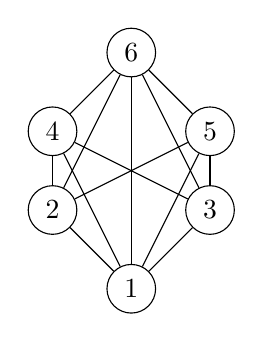
\begin{tikzpicture}
        \node[circle, draw] (u1) at (0, 0) {$1$};
        \node[circle, draw] (u2) at (-1, 1) {$2$};
        \node[circle, draw] (u3) at (1, 1) {$3$};
        \node[circle, draw] (u4) at (-1, 2) {$4$};
        \node[circle, draw] (u5) at (1, 2) {$5$};
        \node[circle, draw] (u6) at (0, 3) {$6$};

        \draw (u1) -- (u2);
        \draw (u1) -- (u3);
        \draw (u1) -- (u4);
        \draw (u1) -- (u5);
        \draw (u1) -- (u6);
        
        \draw (u2) -- (u4);
        \draw (u2) -- (u5);
        \draw (u2) -- (u6);
        
        \draw (u3) -- (u4);
        \draw (u3) -- (u5);
        \draw (u3) -- (u6);

        \draw (u4) -- (u6);
        \draw (u5) -- (u6);
    \end{tikzpicture}
    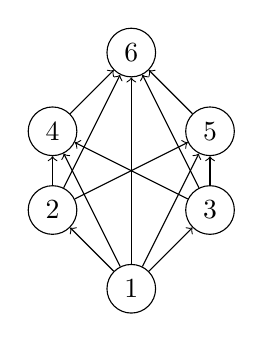
\begin{tikzpicture}
        \node[circle, draw] (u1) at (0, 0) {$1$};
        \node[circle, draw] (u2) at (-1, 1) {$2$};
        \node[circle, draw] (u3) at (1, 1) {$3$};
        \node[circle, draw] (u4) at (-1, 2) {$4$};
        \node[circle, draw] (u5) at (1, 2) {$5$};
        \node[circle, draw] (u6) at (0, 3) {$6$};

        \draw [->] (u1) -> (u2);
        \draw [->] (u1) -> (u3);
        \draw [->] (u1) -> (u4);
        \draw [->] (u1) -> (u5);
        \draw [->] (u1) -> (u6);
        \draw [->] (u2) -> (u4);
        \draw [->] (u2) -> (u5);
        \draw [->] (u2) -> (u6);
        \draw [->] (u3) -> (u4);
        \draw [->] (u3) -> (u5);
        \draw [->] (u3) -> (u6);
        \draw [->] (u4) -> (u6);
        \draw [->] (u5) -> (u6);
    \end{tikzpicture}
    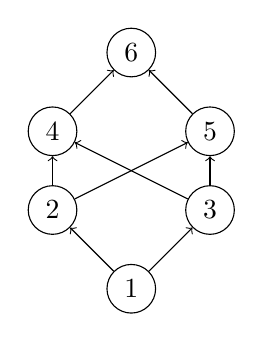
\begin{tikzpicture}
        \node[circle, draw] (u1) at (0, 0) {$1$};
        \node[circle, draw] (u2) at (-1, 1) {$2$};
        \node[circle, draw] (u3) at (1, 1) {$3$};
        \node[circle, draw] (u4) at (-1, 2) {$4$};
        \node[circle, draw] (u5) at (1, 2) {$5$};
        \node[circle, draw] (u6) at (0, 3) {$6$};

        \draw [->] (u1) -> (u2);
        \draw [->] (u1) -> (u3);
        \draw [->] (u2) -> (u4);
        \draw [->] (u2) -> (u5);
        \draw [->] (u3) -> (u4);
        \draw [->] (u3) -> (u5);
        \draw [->] (u4) -> (u6);
        \draw [->] (u5) -> (u6);
    \end{tikzpicture}
    \caption{Ein Vergleichbarkeitsgraph, eine Orientierung davon sowie das Hasse-Diagramm zur Halbordnung der Orientierung.}
\end{figure}

\begin{satz}
    Sei $(V, E)$ ein Vergleichbarkeitsgraph. Dann ist $(V, E)$ perfekt.
\end{satz}
\begin{proof}
    Sei $(V, F)$ eine Orientierung von $(V, E)$. Wir definieren rekursiv eine sogenannte Höhenfunktion $h$ auf den Knoten:
    \begin{align*}
        h : V &\to \N \\
        v &\mapsto \begin{cases}
            0 &v \text{ ist eine Senke}\\
            \max\limits_{wv \in F} h(w) + 1 &\text {sonst}
        \end{cases}
    \end{align*}
    
    Aufgrund der Transitivität und der Antisymmetrie ist der Graph $(V, F)$ zyklenfrei und weil $V$ endlich ist gibt es mindestens eine Senke. Damit ist $h$ wohldefiniert. Definiere $m := \max_{v \in V} h(v)$.

    Für eine Kante $uv \in F$ gilt
    $$h(u) \leq \max\limits_{wv \in F} h(w) = h(v) - 1 < h(v).$$

    Damit ist $h$ also eine zulässige Knotenfärbung für $(V, E)$ mit $m + 1$ vielen Farben.
    
    Zu einem solchen Knoten $v$, bei dem $h(v) = m$ maximal ist, findet man einen Pfad $v =: u_m, \hdots, u_0$ von $v$ zu einer Senke $u_0$ mit $h(u_i) = i\, \forall i \in \N_{\leq m}$, indem man einfach in jedem Schritt einen Zeugen des Maximums in der Definiton von $h$ als nächsten Knoten wählt. Aufgrund der Transitivität von $F$ ist $\{u_i : i \in \N_{\leq m}\}$ sogar eine $m+1$ große Clique.
    
    Es kann also keine größere Clique und keine kleinere Färbung geben und $\chi(G) = m+1 = \omega(G)$. Wegen der Hereditärität ist $(V, E)$ also perfekt.
\end{proof}

\begin{korollar}
    Sei $(V, E)$ ein Vergleichbarkeitsgraph und sei eine Orientierung $(V, E)$ gegeben. Dann kann eine minimale zulässige Färbung $h : V \to \N$, sowie eine maximale Clique in linearer Zeit, also $O(|V| + |F|)$ gefunden werden.
\end{korollar}
\begin{proof}
    
    Die Höhenfunktion $h: V \to \N$ aus dem vorherigen Beweis ist eine zulässige minimale Färbung und kann in linearer Zeit mit Algorithmus \ref{algo:heightfunction} berechnet werden.
    
    \begin{figure}[ht]
        \label{algo:heightfunction}
        \centering
        \begin{minted}{python3}
def compute_height(G: DirectedGraph) -> dict[Vertex, int]:
    h = dict()
    unset_inneighbor_count = {u: u.indegree for u in G.vertices}
    
    def DFS(u: Vertex):
        unset_inneighbor_count[u] -= 1
        if unset_inneighbor_count[u] == 0:
            h[u] = max(h[v] for v in u.in_neighbors) + 1
            for w in u.out_neighbors:
                DFS(w)
        
    for u in G.vertices:
        if u.indegree == 0:
            h[u] = 0
            for v in u.out_neighbors:
                DFS(v)
    
    return h
        \end{minted}
        \caption{Pseudo-Pseudo-Code zur Berechnung der Höhenfunktion. Details zur Implementierung gibt es in Appendix \ref{appendix:code}.}
    \end{figure}
    
    Der Algorithmus läuft über eine Tiefensuche \emph{(eng. Depth-First-Search, DFS)}, wobei $h$ für einen Knoten erst berechnet wird, wenn $h$ für alle Ausgang-Nachbaren bereits berechnet sind. In \verb|unset_outneighbor_count[u]| wird absteigend gezählt, wie oft die Funktion \verb|DFS| für einen Knoten \verb|u| aufgerufen wurde. Sobald \verb|DFS| von jedem seiner Ausgang-Nachbaren aufgerufen wurde und \verb|unset_outneighbor_count[u]| $= 0$ ist sicher, das $h$ für alle Ausgang-Nachbaren von \verb|u| berechnet wurde.
    
    \verb|DFS| wird pro Kante einmal aufgerufen und pro (nicht Senke-)Knoten $u$ wird einmal der Teil innerhalb der \verb|if|-Abfrage ausgeführt, welcher $O(Ausgrad(u))$ für das Maximum und $O(Ingrad(u))$ für das Aufrufen von \verb|DFS| braucht.
    
    Die Vorbereitung von \verb|unset_outneighbor_count| sowie das Durchlaufen der Knoten auf der Suche nach den Senken braucht jeweils $O(|V|)$. Insgesamt braucht der Algorithmus also $O(2\cdot|V| + 3\cdot|F|) = O(|V| + |F|)$ viel Zeit.

    \begin{figure}[ht]
        \label{algo:clique}
        \centering
        \begin{minted}{python3}
def find_path(G: DirectedGraph) -> list[Vertex]:
    h = compute_height(G)

    max_vertex = max(h, key=h.get)
    
    current_vertex = max_vertex
    path = [max_vertex]
    while h[current_vertex] > 0:
        for neighbor in current_vertex.in_neighbors:
            if h[neighbor] == h[current_vertex] - 1:
                current_vertex = neighbor
                break
        path.append(current_vertex)

    path.reverse()
    return path
        \end{minted}
        \caption{Pseudo-Pseudo-Code zur Berechnung einer Clique.}
    \end{figure}

\end{proof}
    
\begin{figure}[ht]
    \label{fig:comparability_graph}
    \centering
    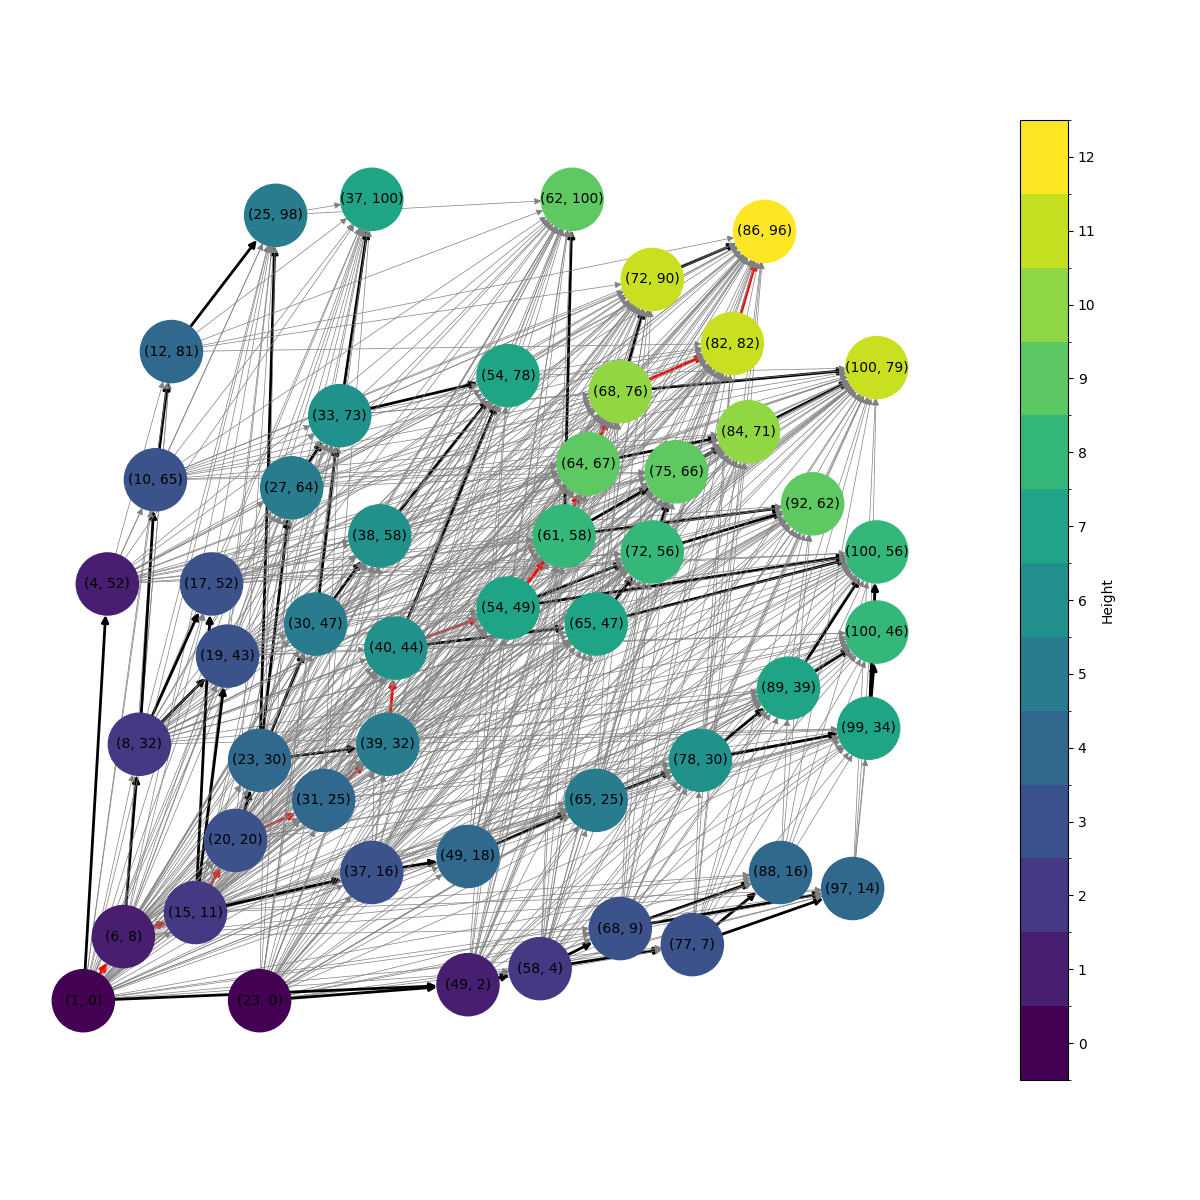
\includegraphics[width=\textwidth]{figures/comparability_graph.png}
    \caption{Beispiel für (die Orientierung eines) Vergleichbarkeitsgraphen. Die Knoten sind Zahlenpaare und $(a, b) < (c, d) :\Leftrightarrow a < c \wedge b < d$. Die Farbe der Knoten entspricht der Höhe $h$. Die dick eingezeichneten Kanten sind jene, wo der Höhenunterschied nur 1 ist. In Rot ist ein maximaler Pfad (und damit eine maximale Clique) eingezeichnet.}
\end{figure}
    

\begin{satz}
    Der schwache Perfekte-Graphen-Satz: Sei $G = (V, E)$ ein Graph. Dann sind die folgenden Aussagen äquivalent:
    \begin{align}
        \omega(G_A) &= \chi(G_A) &(\forall A \subset V) \tag{P1}\label{eq:P1}\\
        \omega(\overline{G_A}) &= \chi(\overline{G_A}) &(\forall A \subset V) \tag{P2}\label{eq:P2}\\
        \omega(G_A) \cdot \omega(\overline{G_A}) &\geq |A| &(\forall A \subset V) \tag{P3}\label{eq:P3}
    \end{align}
    Insbesondere ist $G$ perfekt genau dann wenn $\overline G$ perfekt ist.
\end{satz}
\begin{proof}
    (\ref{eq:P1}) $\Rightarrow$ (\ref{eq:P3}): Sei $A \subset V$ beliebig. Angenommen wir färben $G_A$ mit $\omega(G_A)$ Farben. Jede Farbe kann von höchstens $\omega(\overline{G_A})$ vielen Knoten angenommen werden, da gleichgefärbte Knoten eine Clique im Komplement bilden. Über alle Farben aufsummiert ergibt sich $\omega(G_A) \cdot \omega(\overline{G_A}) \geq |A|$.

    (\ref{eq:P3}) $\Rightarrow$ (\ref{eq:P1}): \todo{Finish Proof}
\end{proof}

Die zylischen Graphen $C_n$ für $n \in \N, n > 3, n$ ungerade sind keine perfekten Graphen, da $\chi(C_n) = 3 \neq 2 = \omega(C_n)$. Da all deren induzierte Teilgraphen perfekt sind, stellen diese Graphen (auch \emph{ungerade Löcher} genannt) und deren Komplemente (\emph{ungerade Anti-Löcher}) in gewisserweise minimale Gegenbeispiele für die Perfektheit dar. Es stellt sich in natürlicherweise die Frage: Gibt es noch andere Graphen, die nicht perfekt sind, aber alle echten induzierten Teilgraphen perfekt sind?

Bereits im März 1960 stellt Claude Berge diese Frage und vermutet, dass dies alle sind.\cite{das_Buch} Er behielt damit Recht, den Beweis lieferten Maria Chudnovsky, Neil Robertson, Paul Seymour und Robin Thomas\cite{chudnovsky2002strongperfectgraphtheorem} erst viel später im Jahr 2002.

Dieses Resultat führt zu einer \emph{forbidden minor}-Charakterisierung der Perfektheit, ähnlich zu planaren Graphen mit $K_5$ und $K_{3,3}$:

\begin{satz}
    Der starke Perfekte-Graphen-Satz: Ein Graph $G = (V, E)$ ist genau dann perfekt, wenn $G$ keinen induzierten Teilgraphen isomorph zu $C_n$ oder $\overline{C_n}$ für $n \in \N, n > 3, n$ ungerade hat.
\end{satz}


\todo{
Ausblick:
    Wir schauen uns spezielle Klassen von perfekten Graphen und Algorithmen darauf an.
        - Triangulated Graphs
        - ...
}

\end{document}